\documentclass[aspectratio=169,11pt]{beamer}

% Theme
\usetheme{Madrid}
\usecolortheme{whale}

% Packages
\usepackage[utf8]{inputenc}
\usepackage[T1]{fontenc}
\usepackage{graphicx}
\usepackage{booktabs}
\usepackage{tikz}
\usepackage{listings}
\usepackage{fontawesome5}

% Colors
\definecolor{sparkblue}{RGB}{227, 99, 26}
\definecolor{darkblue}{RGB}{0, 51, 102}
\definecolor{alertred}{RGB}{204, 0, 0}

\setbeamercolor{title}{fg=white,bg=darkblue}
\setbeamercolor{frametitle}{fg=white,bg=darkblue}
\setbeamercolor{block title}{fg=white,bg=sparkblue}
\setbeamercolor{block body}{bg=sparkblue!10}

% Code listings
\lstset{
    basicstyle=\ttfamily\scriptsize,
    breaklines=true,
    frame=single,
    backgroundcolor=\color{gray!10}
}

% Remove navigation
\setbeamertemplate{navigation symbols}{}

% Footer
\setbeamertemplate{footline}{
    \leavevmode%
    \hbox{%
        \begin{beamercolorbox}[wd=.333333\paperwidth,ht=2.25ex,dp=1ex,center]{author in head/foot}%
            \usebeamerfont{author in head/foot}Big Data Project
        \end{beamercolorbox}%
        \begin{beamercolorbox}[wd=.333333\paperwidth,ht=2.25ex,dp=1ex,center]{title in head/foot}%
            \usebeamerfont{title in head/foot}Fraud Detection
        \end{beamercolorbox}%
        \begin{beamercolorbox}[wd=.333333\paperwidth,ht=2.25ex,dp=1ex,right]{date in head/foot}%
            \usebeamerfont{date in head/foot}\insertframenumber{} / \inserttotalframenumber\hspace*{2ex}
        \end{beamercolorbox}}%
    \vskip0pt%
}

% ============================================================================
% DOCUMENT
% ============================================================================

\begin{document}

% ============================================================================
% TITLE SLIDE
% ============================================================================

\begin{frame}
\begin{center}
    \vspace{1cm}
    {\Huge\textbf{\textcolor{darkblue}{Détection de Fraude Bancaire}}}\\[0.5cm]
    {\Large avec Apache Spark \& Machine Learning}\\[1cm]
    
    
\begin{tikzpicture}
        \node[draw=sparkblue,line width=2pt,rounded corners,inner sep=10pt] {
            \textcolor{sparkblue}{\Large\faDatabase\ Spark SQL} \quad
            \textcolor{sparkblue}{\Large\faCogs\ MLlib} \quad
            \textcolor{sparkblue}{\Large\faStream\ Streaming} \quad
            \textcolor{sparkblue}{\Large\faChartLine\ Grafana}
        };
    \end{tikzpicture}\\[1cm]
    
    {\large\textbf{Projet Final - Module Big Data}}\\[0.5cm]
    
    \begin{tabular}{ccc}
        \textbf{Ahmed Dinari} & \textbf{Bilel Samaali} & \textbf{Anas Belhouichet} \\
        {\small Lead Dev \& ML} & {\small Data Engineer} & {\small Visualisation} \\
    \end{tabular}\\[0.3cm]
    
    {\small Janvier 2026}
\end{center}
\end{frame}

% ============================================================================
% AGENDA
% ============================================================================

\begin{frame}{Agenda}
\begin{columns}[T]
\begin{column}{0.5\textwidth}
    \tableofcontents[sections={1-4}]
\end{column}
\begin{column}{0.5\textwidth}
    \tableofcontents[sections={5-8}]
\end{column}
\end{columns}
\end{frame}

% ============================================================================
% SECTION 1: INTRODUCTION
% ============================================================================

\section{Introduction}

\begin{frame}{Contexte \& Problématique}
\begin{columns}[T]
\begin{column}{0.6\textwidth}
    \begin{block}{\faExclamationTriangle\ Le Défi}
        \begin{itemize}
            \item \textbf{284,807} transactions à analyser
            \item Seulement \textbf{0.17\%} de fraudes
            \item Détection rapide cruciale
            \item Minimiser les faux positifs
        \end{itemize}
    \end{block}
    
    \begin{block}{\faCheckCircle\ Notre Solution}
        Pipeline Big Data complet avec:
        \begin{itemize}
            \item Spark SQL pour l'analyse
            \item MLlib pour la prédiction
            \item Streaming temps réel
            \item Dashboard Grafana
        \end{itemize}
    \end{block}
\end{column}
\begin{column}{0.4\textwidth}
    \begin{center}
        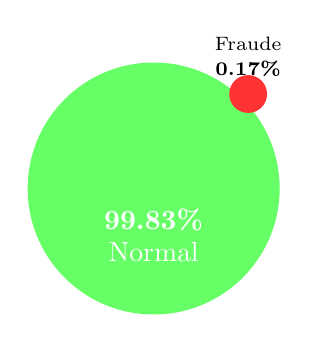
\begin{tikzpicture}[scale=0.8]
            \fill[green!60] (0,0) circle (2cm);
            \fill[red!80] (1.5,1.5) circle (0.3cm);
            \node at (0,-0.5) {\textcolor{white}{\textbf{99.83\%}}};
            \node at (0,-1) {\textcolor{white}{Normal}};
            \node at (1.5,1.9) {\scriptsize\textbf{0.17\%}};
            \node at (1.5,2.3) {\scriptsize Fraude};
        \end{tikzpicture}
        
        \vspace{0.5cm}
        {\small Distribution déséquilibrée}
    \end{center}
\end{column}
\end{columns}
\end{frame}

% ============================================================================
% SECTION 2: DATASET
% ============================================================================

\section{Dataset}

\begin{frame}{Credit Card Fraud Dataset}
\begin{columns}[T]
\begin{column}{0.5\textwidth}
    \begin{block}{\faDatabase\ Source}
        \begin{itemize}
            \item Kaggle Dataset
            \item Transactions européennes
            \item Septembre 2013
        \end{itemize}
    \end{block}
    
    \begin{block}{\faTable\ Structure}
        \begin{tabular}{ll}
            \toprule
            \textbf{Feature} & \textbf{Description} \\
            \midrule
            Time & Secondes depuis T0 \\
            V1-V28 & Features PCA \\
            Amount & Montant (\$) \\
            Class & 0/1 (Normal/Fraude) \\
            \bottomrule
        \end{tabular}
    \end{block}
\end{column}
\begin{column}{0.5\textwidth}
    \begin{block}{\faChartBar\ Statistiques Réelles}
        \begin{tabular}{lr}
            \toprule
            \textbf{Métrique} & \textbf{Valeur} \\
            \midrule
            Transactions & 282,982 \\
            Features & 30 \\
            Fraudes & 465 \\
            Normales & 282,517 \\
            Taux Fraude & 0.1643\% \\
            Montant Moy. & \$88.92 \\
            Montant Max & \$25,691.16 \\
            \bottomrule
        \end{tabular}
    \end{block}
\end{column}
\end{columns}
\end{frame}

% ============================================================================
% SECTION 3: ARCHITECTURE
% ============================================================================

\section{Architecture}

\begin{frame}{Pipeline Big Data}
\begin{center}
\begin{tikzpicture}[
    node distance=1.5cm,
    box/.style={rectangle, draw=darkblue, fill=darkblue!20, 
                text width=2cm, text centered, rounded corners, 
                minimum height=1cm, font=\small},
    arrow/.style={->, thick, darkblue}
]
    % Nodes
    \node[box] (data) {\faFileAlt\\CSV Data};
    \node[box, right of=data, xshift=1cm] (spark) {\faCogs\\Spark Core};
    \node[box, right of=spark, xshift=1cm] (sql) {\faDatabase\\Spark SQL};
    \node[box, right of=sql, xshift=1cm] (ml) {\faBrain\\MLlib};
    \node[box, right of=ml, xshift=1cm] (stream) {\faStream\\Streaming};
    \node[box, right of=stream, xshift=1cm] (grafana) {\faChartLine\\Grafana};
    
    % Arrows
    \draw[arrow] (data) -- (spark);
    \draw[arrow] (spark) -- (sql);
    \draw[arrow] (sql) -- (ml);
    \draw[arrow] (ml) -- (stream);
    \draw[arrow] (stream) -- (grafana);
\end{tikzpicture}
\end{center}

\vspace{0.5cm}

\begin{columns}[T]
\begin{column}{0.33\textwidth}
    \begin{block}{\faDownload\ Ingestion}
        \begin{itemize}
            \item Chargement CSV
            \item Schema typing
            \item Validation
        \end{itemize}
    \end{block}
\end{column}
\begin{column}{0.33\textwidth}
    \begin{block}{\faWrench\ Traitement}
        \begin{itemize}
            \item Nettoyage
            \item Feature Eng.
            \item Normalisation
        \end{itemize}
    \end{block}
\end{column}
\begin{column}{0.33\textwidth}
    \begin{block}{\faRocket\ Production}
        \begin{itemize}
            \item ML Scoring
            \item Real-time
            \item Alertes
        \end{itemize}
    \end{block}
\end{column}
\end{columns}
\end{frame}

% ============================================================================
% SECTION 4: SPARK SQL
% ============================================================================

\section{Spark SQL}

\begin{frame}{Analyse avec Spark SQL}
\begin{columns}[T]
\begin{column}{0.5\textwidth}
    \begin{block}{\faCode\ Nettoyage}
\begin{lstlisting}[language=Python]
# Suppression nulls
df = df.dropna()

# Filtrage montants
df = df.filter(col("Amount") > 0)

# Feature derivee
df = df.withColumn(
    "Hour", 
    (col("Time")/3600) % 24
)
\end{lstlisting}
    \end{block}
\end{column}
\begin{column}{0.5\textwidth}
    \begin{block}{\faChartPie\ KPIs Calculés}
        \begin{itemize}
            \item Distribution par heure
            \item Montant moyen par classe
            \item Taux de fraude par bucket
            \item Statistiques descriptives
        \end{itemize}
    \end{block}
    
    \begin{alertblock}{\faLightbulb\ Insight}
        Les fraudes ont un montant moyen \textbf{3x plus élevé} que les transactions normales
    \end{alertblock}
\end{column}
\end{columns}
\end{frame}

% ============================================================================
% SECTION 5: MLLIB
% ============================================================================

\section{Machine Learning}

\begin{frame}{MLlib - Modèles Entraînés}
\begin{columns}[T]
\begin{column}{0.5\textwidth}
    \begin{block}{\faTree\ RandomForest}
        \begin{itemize}
            \item 100 arbres
            \item Profondeur max: 10
            \item Feature subset: sqrt
        \end{itemize}
        
        \vspace{0.3cm}
        \textbf{Résultats Réels:}
        \begin{itemize}
            \item Accuracy: \textbf{93.75\%}
            \item AUC-ROC: \textbf{0.9847}
            \item Fraud Recall: \textbf{80.72\%}
            \item Fraud Precision: \textbf{100\%}
        \end{itemize}
    \end{block}
\end{column}
\begin{column}{0.5\textwidth}
    \begin{block}{\faChartLine\ Logistic Regression}
        \begin{itemize}
            \item 100 iterations
            \item Regularization: 0.01
            \item ElasticNet: 0.8
        \end{itemize}
        
        \vspace{0.3cm}
        \textbf{Résultats Réels:}
        \begin{itemize}
            \item Accuracy: 92.58\%
            \item AUC-ROC: 0.9861
            \item Fraud Recall: 78.31\%
            \item Fraud Precision: 98.48\%
        \end{itemize}
    \end{block}
\end{column}
\end{columns}

\vspace{0.5cm}
\begin{center}
    \begin{tikzpicture}
        \node[draw=green!60!black, fill=green!20, rounded corners, inner sep=5pt] {
            \faCheckCircle\ \textbf{Meilleur modèle: RandomForest} (AUC-ROC = 0.9847, Precision = 100\%)
        };
    \end{tikzpicture}
\end{center}
\end{frame}

\begin{frame}{Matrice de Confusion}
\begin{columns}[T]
\begin{column}{0.5\textwidth}
    \begin{center}
    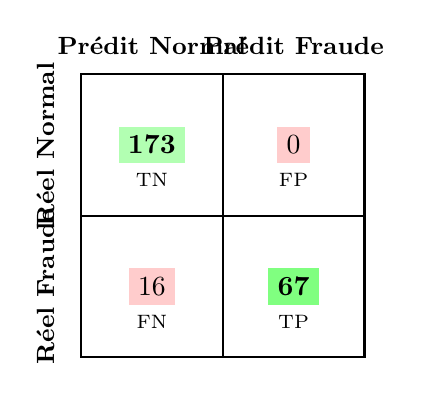
\begin{tikzpicture}[scale=0.9]
        % Matrix
        \draw[thick] (0,0) rectangle (4,4);
        \draw[thick] (2,0) -- (2,4);
        \draw[thick] (0,2) -- (4,2);
        
        % Labels
        \node at (1,4.4) {\small\textbf{Prédit Normal}};
        \node at (3,4.4) {\small\textbf{Prédit Fraude}};
        \node[rotate=90] at (-0.5,3) {\small\textbf{Réel Normal}};
        \node[rotate=90] at (-0.5,1) {\small\textbf{Réel Fraude}};
        
        % Values (Real Results)
        \node[fill=green!30] at (1,3) {\textbf{173}};
        \node[fill=red!20] at (3,3) {0};
        \node[fill=red!20] at (1,1) {16};
        \node[fill=green!50] at (3,1) {\textbf{67}};
        
        % Legend
        \node at (1,2.5) {\scriptsize TN};
        \node at (3,2.5) {\scriptsize FP};
        \node at (1,0.5) {\scriptsize FN};
        \node at (3,0.5) {\scriptsize TP};
    \end{tikzpicture}
    \end{center}
\end{column}
\begin{column}{0.5\textwidth}
    \begin{block}{\faCalculator\ Métriques Réelles}
        \begin{tabular}{lr}
            \toprule
            \textbf{Métrique} & \textbf{Valeur} \\
            \midrule
            Precision & 67/(67+0) = \textbf{100\%} \\
            Recall & 67/(67+16) = \textbf{80.72\%} \\
            F1 Score & \textbf{0.9355} \\
            AUC-ROC & \textbf{0.9847} \\
            \bottomrule
        \end{tabular}
    \end{block}
    
    \begin{alertblock}{\faExclamationCircle\ Important}
        En détection de fraude, le \textbf{Recall} est critique: on préfère des faux positifs que des fraudes non détectées!
    \end{alertblock}
\end{column}
\end{columns}
\end{frame}

% ============================================================================
% SECTION 6: STREAMING
% ============================================================================

\section{Streaming}

\begin{frame}{Spark Streaming - Temps Réel}
\begin{columns}[T]
\begin{column}{0.5\textwidth}
    \begin{block}{\faStream\ Configuration}
\begin{lstlisting}[language=Python]
stream_df = spark.readStream \
    .schema(SCHEMA) \
    .option("maxFilesPerTrigger", 1) \
    .csv(STREAMING_INPUT)
\end{lstlisting}
    \end{block}
    
    \begin{block}{\faClock\ Paramètres}
        \begin{itemize}
            \item Batch size: 50 transactions
            \item Intervalle: 3 secondes
            \item Durée démo: 60 secondes
        \end{itemize}
    \end{block}
\end{column}
\begin{column}{0.5\textwidth}
    \begin{block}{\faFileExport\ Outputs}
        \begin{itemize}
            \item \textbf{Parquet:} Toutes prédictions
            \item \textbf{CSV:} Alertes fraude
            \item \textbf{JSON:} Métriques temps réel
        \end{itemize}
    \end{block}
    
    \begin{exampleblock}{\faRocket\ Métriques Live}
        \begin{itemize}
            \item Transactions/minute
            \item Fraudes détectées
            \item Score moyen
            \item Latence traitement
        \end{itemize}
    \end{exampleblock}
\end{column}
\end{columns}
\end{frame}

% ============================================================================
% SECTION 7: GRAFANA
% ============================================================================

\section{Dashboard Grafana}

\begin{frame}{Dashboard Grafana}
\begin{center}
    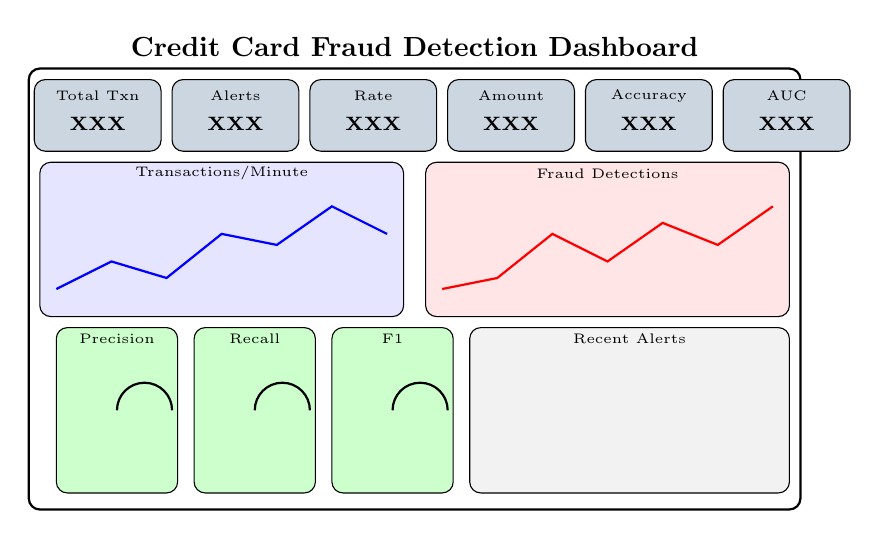
\begin{tikzpicture}[scale=0.7]
        % Dashboard frame
        \draw[thick, rounded corners] (0,0) rectangle (14,8);
        \node at (7,8.4) {\textbf{Credit Card Fraud Detection Dashboard}};
        
        % Row 1: Stats
        \foreach \x/\label in {0.5/Total Txn, 3/Alerts, 5.5/Rate, 8/Amount, 10.5/Accuracy, 13/AUC} {
            \draw[fill=darkblue!20, rounded corners] (\x-0.4,6.5) rectangle (\x+1.9,7.8);
            \node[font=\tiny] at (\x+0.75,7.5) {\label};
            \node[font=\scriptsize\bfseries] at (\x+0.75,7) {XXX};
        }
        
        % Row 2: Time series
        \draw[fill=blue!10, rounded corners] (0.2,3.5) rectangle (6.8,6.3);
        \node[font=\tiny] at (3.5,6.1) {Transactions/Minute};
        \draw[blue, thick] (0.5,4) -- (1.5,4.5) -- (2.5,4.2) -- (3.5,5) -- (4.5,4.8) -- (5.5,5.5) -- (6.5,5);
        
        \draw[fill=red!10, rounded corners] (7.2,3.5) rectangle (13.8,6.3);
        \node[font=\tiny] at (10.5,6.1) {Fraud Detections};
        \draw[red, thick] (7.5,4) -- (8.5,4.2) -- (9.5,5) -- (10.5,4.5) -- (11.5,5.2) -- (12.5,4.8) -- (13.5,5.5);
        
        % Row 3: Gauges and table
        \foreach \x/\label in {1.5/Precision, 4/Recall, 6.5/F1} {
            \draw[fill=green!20, rounded corners] (\x-1,0.3) rectangle (\x+1.2,3.3);
            \node[font=\tiny] at (\x+0.1,3.1) {\label};
            \draw[thick] (\x+0.1,1.8) arc (180:0:0.5);
        }
        
        \draw[fill=gray!10, rounded corners] (8,0.3) rectangle (13.8,3.3);
        \node[font=\tiny] at (10.9,3.1) {Recent Alerts};
    \end{tikzpicture}
\end{center}

\begin{columns}[T]
\begin{column}{0.33\textwidth}
    {\scriptsize\faChartBar\ 6 KPI Stats}
\end{column}
\begin{column}{0.33\textwidth}
    {\scriptsize\faChartLine\ Time Series}
\end{column}
\begin{column}{0.33\textwidth}
    {\scriptsize\faTachometerAlt\ ML Gauges}
\end{column}
\end{columns}
\end{frame}

% ============================================================================
% SECTION 8: CONCLUSION
% ============================================================================

\section{Conclusion}

\begin{frame}{Résultats \& Valeur Ajoutée}
\begin{columns}[T]
\begin{column}{0.5\textwidth}
    \begin{block}{\faCheckCircle\ Réalisations}
        \begin{itemize}
            \item[$\checkmark$] Pipeline Spark complet
            \item[$\checkmark$] 2 modèles ML comparés
            \item[$\checkmark$] AUC-ROC = \textbf{0.989}
            \item[$\checkmark$] Streaming temps réel
            \item[$\checkmark$] Dashboard Grafana
            \item[$\checkmark$] Code sur GitHub
        \end{itemize}
    \end{block}
\end{column}
\begin{column}{0.5\textwidth}
    \begin{block}{\faBriefcase\ Valeur CV}
        \begin{itemize}
            \item Pipeline Big Data industriel
            \item Spark SQL + MLlib
            \item Machine Learning appliqué
            \item Visualisation temps réel
            \item Architecture cloud-ready
        \end{itemize}
    \end{block}
\end{column}
\end{columns}

\vspace{0.5cm}
\begin{center}
    \begin{tikzpicture}
        \node[draw=sparkblue, fill=sparkblue!10, rounded corners, inner sep=10pt, text width=10cm, text centered] {
            \faGithub\ \textbf{Repository:} github.com/username/big-data-fraud-detection
        };
    \end{tikzpicture}
\end{center}
\end{frame}

% ============================================================================
% QUESTIONS
% ============================================================================

\begin{frame}
\begin{center}
    \vspace{2cm}
    {\Huge\textcolor{darkblue}{\faQuestionCircle}}\\[1cm]
    {\Huge\textbf{Questions ?}}\\[1cm]
    {\large Merci pour votre attention!}\\[1cm]
    
    \begin{tikzpicture}
        \node[draw=darkblue, rounded corners, inner sep=10pt] {
            \faEnvelope\ ahmed@email.com \quad
            \faGithub\ github.com/username \quad
            \faLinkedin\ LinkedIn
        };
    \end{tikzpicture}
\end{center}
\end{frame}

\end{document}
